\documentclass{article}\usepackage[]{graphicx}\usepackage[]{color}
% maxwidth is the original width if it is less than linewidth
% otherwise use linewidth (to make sure the graphics do not exceed the margin)
\makeatletter
\def\maxwidth{ %
  \ifdim\Gin@nat@width>\linewidth
    \linewidth
  \else
    \Gin@nat@width
  \fi
}
\makeatother

\definecolor{fgcolor}{rgb}{0.345, 0.345, 0.345}
\newcommand{\hlnum}[1]{\textcolor[rgb]{0.686,0.059,0.569}{#1}}%
\newcommand{\hlstr}[1]{\textcolor[rgb]{0.192,0.494,0.8}{#1}}%
\newcommand{\hlcom}[1]{\textcolor[rgb]{0.678,0.584,0.686}{\textit{#1}}}%
\newcommand{\hlopt}[1]{\textcolor[rgb]{0,0,0}{#1}}%
\newcommand{\hlstd}[1]{\textcolor[rgb]{0.345,0.345,0.345}{#1}}%
\newcommand{\hlkwa}[1]{\textcolor[rgb]{0.161,0.373,0.58}{\textbf{#1}}}%
\newcommand{\hlkwb}[1]{\textcolor[rgb]{0.69,0.353,0.396}{#1}}%
\newcommand{\hlkwc}[1]{\textcolor[rgb]{0.333,0.667,0.333}{#1}}%
\newcommand{\hlkwd}[1]{\textcolor[rgb]{0.737,0.353,0.396}{\textbf{#1}}}%
\let\hlipl\hlkwb

\usepackage{framed}
\makeatletter
\newenvironment{kframe}{%
 \def\at@end@of@kframe{}%
 \ifinner\ifhmode%
  \def\at@end@of@kframe{\end{minipage}}%
  \begin{minipage}{\columnwidth}%
 \fi\fi%
 \def\FrameCommand##1{\hskip\@totalleftmargin \hskip-\fboxsep
 \colorbox{shadecolor}{##1}\hskip-\fboxsep
     % There is no \\@totalrightmargin, so:
     \hskip-\linewidth \hskip-\@totalleftmargin \hskip\columnwidth}%
 \MakeFramed {\advance\hsize-\width
   \@totalleftmargin\z@ \linewidth\hsize
   \@setminipage}}%
 {\par\unskip\endMakeFramed%
 \at@end@of@kframe}
\makeatother

\definecolor{shadecolor}{rgb}{.97, .97, .97}
\definecolor{messagecolor}{rgb}{0, 0, 0}
\definecolor{warningcolor}{rgb}{1, 0, 1}
\definecolor{errorcolor}{rgb}{1, 0, 0}
\newenvironment{knitrout}{}{} % an empty environment to be redefined in TeX

\usepackage{alltt}
\usepackage{graphicx}
\usepackage[top=1.00in, bottom=1.0in, left=1.1in, right=1.1in]{geometry}
\renewcommand{\baselinestretch}{1.1}
\IfFileExists{upquote.sty}{\usepackage{upquote}}{}
\begin{document}

\section{The main question: Are PMM's appropriate for my data structure?}

\subsection{What is my desired model and data structure?}
I'd like to use a repeat measure PMM as detailed in chapter 11 of Modern Phylogenetic Comparative Methods and the application in Evolutionary Biology (de Villemeruil & Nakagawa, 2014).\\

I am trying to predict the time between flowering and leaf expansion (FLS) for 23 species from Harvard Forest as a function of their pollination syndrome, minimum precipitation across their range, day of flowering with all two way interactions and accounting for phylogeny.\\

The possible problem (the point of this treatment is to determine whether or not this is a problem) is all of my variable are recorded at different levels of organization.

\begin{itemize}
\item FLS- repeat measure across 3-5 individuals per species over 15 year.\\
\item pollination syndrome- one value/species\\
\item minimum precipitation-one value/species\\
\item flowering time: repeat measure across 3-5 individuals per species over 15 year.\\
\item See the head of the data below:\\
\end{itemize}
\begin{knitrout}
\definecolor{shadecolor}{rgb}{0.969, 0.969, 0.969}\color{fgcolor}\begin{kframe}
\begin{verbatim}
##   species               name fopn.jd min_precip pol funct.fls
## 1    ACPE Acer_pensylvanicum     136         24   0         9
## 2    ACPE Acer_pensylvanicum     129         24   0        19
## 3    ACPE Acer_pensylvanicum     138         24   0        16
## 4    ACPE Acer_pensylvanicum     130         24   0        12
## 5    ACPE Acer_pensylvanicum     135         24   0         9
## 6    ACPE Acer_pensylvanicum     138         24   0         7
\end{verbatim}
\end{kframe}
\end{knitrout}
I standardize (z-score) all predictors for comparison.\\

This model I have been using and would like to continue to do so:\\
FLS = pol+flowing+precip+precip:flo+precip:pol+pol:flowing+(1|name)+(1|tree.id/species),covranef = list(name= A))\\  

The covariance structure to the random effect "name" accounts for phylogentic correlations in the inter-specific residuals. The tree.id/species random effect is in this case "an individual/species-specific" term accounting for variability in the estimate not attributed to phylogeny. This all seems well and good until we encounter the following line from de Villemeruil & Nakagawa:\\

`` As a comparative biologist, the reader would most likely be interested in the between species slope. If co factor x (ie my predictor), only contains one value per species, then there is no problem... Things are slightly more complicated  using individual measurements in x, but it is still possible to obtain between species and within species slopes using a technique called within group centering  (Davis et al 1961, van de Pol and Wright 2009). This separates x into two components, the containing the species level mean, and one containing species level variability."

Here's the thing. I am not precisely interested in estimating the within species slope. Rather, I'd like to estimate the between species slope, but have the model ``account" for the within species variation but not necessarily estimate it explicitly.

Yet, the quote above would suggest the proper model is:\\

FLS = pol+meanflotime+varflotime+precip+all 2 way interactions +(1|name)+(1|species) covranef = list(name= A))\\

When I run this model, it generates huge credible interval for all predictors, and only mean flowering time matters. This is contrary to all other models I've ever run on this data set and other hysteranthy data, as well as my biological expectation. (eg I am fairly certain pollination syndrome matters.)\\

\section{So what went wrong?}
Why are these answers so different? Nacho and I discussed this. Neither of us were sure. Nacho thinks maybe that what seems important is these data are changing to phylogenetic covariance structure in the residuals.
\begin{itemize}
\item Suggeston: Because the variables aren't balanced (ie Acer rubrum has 100 FLS and flowering time estimates and other species have as few as 40), this is biasing the phylogeny through weighting it differently.
\item But here's what I'm thinking: To me this would be a problem with a lack of balance in the response variable more than the predictor because the model is pooling only on intercepts. I don't see why partitioning within and among species variance in a \emph{predictor}, would help this.
\end{itemize}

\section{A foray into qualitative model comparison}
So we don't really know what is wrong. But if we follow the lead that the phylogenetic inaccuracies are driving the giant differences between the models, it follows accordingly that removing the phylogeny and covariance structures entirely should bring he models closer together.\\

So I ran 4 models. 1. meanfloweringtime w/ phylo (no vary predictors). 2. meanfloweringtime w/o phylo (no vary predictors). 3. original model w/ phylo (vary predictors). 4. original model w/o phylo (vary predictors. *Note: for simplicitly of comparision I didn't include the flowering variationterm in this graphic, just mean flowering time per species. When I did run that full model, there was also a much weaker effect of flowering time variation, but the other predictors didn't change.* Here is a comparative mu plot:\\

 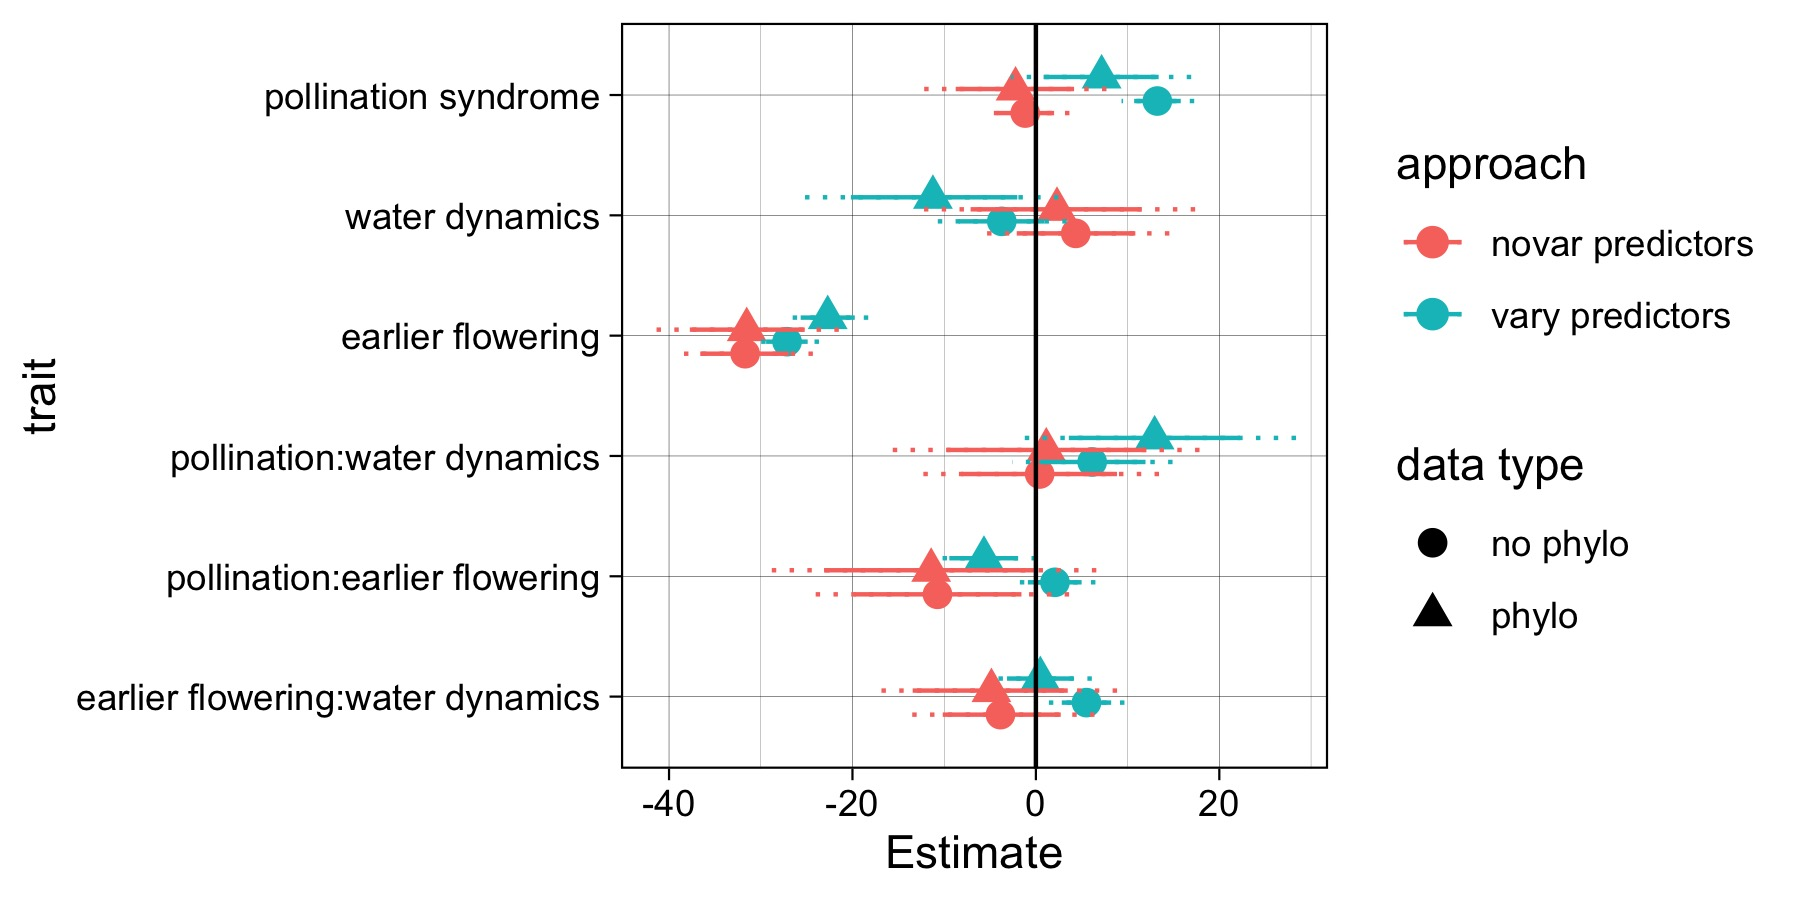
\includegraphics[width=\textwidth]{Uhoh_best.jpeg} 
    \caption{\textbf{As you can see here, even when ignoring the phylogeny the mean flowering time and original models are very different. Adding the phylogeny changes them a bit, but each one is still more similar to itself with or without the phylogeny }.}


\section{Take-away:}
I think it's still important to understand why these two approaches yield such different estimates. However, because my original model with and without the phylogeny still give estimates that are FAR more qualitatively similar to each other than either of the mean flowering time models, I don't feel like my original formulation is wrong per say, just different.\\

I would love to hear your thoughts on this.





\end{document}
